% file: 3-7-sssp/bellman-ford-two-negative-cycles.tex

\documentclass[tikz]{standalone}
\usetikzlibrary{shapes, positioning, decorations.pathmorphing}

\begin{document}
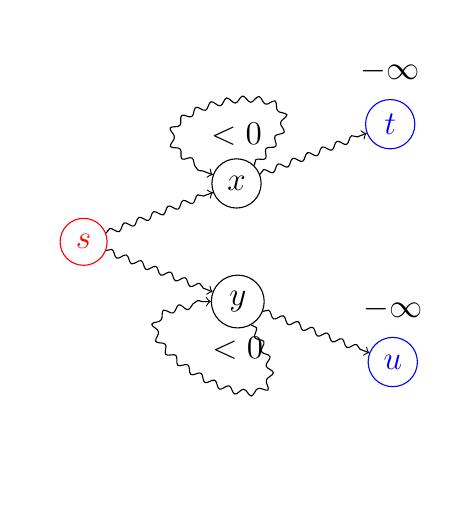
\begin{tikzpicture}[every node/.style = {draw, circle, minimum size = 8pt, font = \large},
    node distance = 0.30cm and 1.5cm,
    every edge/.style = {draw, ->, decorate, decoration = {snake, amplitude = .4mm, segment length = 2mm, post length = 1mm}}]
  \node (s) [red] {$s$};

  \node (x) [above right = of s, label = {[above = -6pt]: $< 0$}] {$x$};
  \node (t) [above right = of x, blue, label = {[above = -6pt]: $-\infty$}] {$t$};

  \node (y) [below right = of s, label = {[below = 12pt]: $< 0$}] {$y$};
  \node (u) [below right = of y, blue, label = {[above = -6pt]: $-\infty$}] {$u$};

  \path (s) edge (x)
	    edge (y)
	(x) edge[out = 45, in = 160, looseness = 10] (x)
	    edge (t)
	(y) edge[out = -60, in = -180, looseness = 10] (y)
	    edge (u);
\end{tikzpicture}
\end{document}
